\chapter{Results}
Examining the changes in orchestration of brain function through hierarchy induced by ayahuasca and DMT
allows for a deeper look into the mechanisms of psychedelic action, adding nuance to existing theories and bridging 
the gap between the profound alterations in consciousness resulting from psychedelics and their biological effects. Furthermore, we aimed to add further evidence to a recent unified model of psychedelic action on the brain \parencite{Carhart-Harris2019a}.
Figure \ref{fig:overview} describes the overall framework employed in this study. Participants were scanned and BOLD timeseries for each region of a coarse-grained parcellation, the Mindboggle-modified Desikan-Killiany with subcortical regions (DK80), were extracted. Production entropy is estimated via irreversibility by exploiting the fact that hierarchical processes necessarily produce entropy. Irreversibility in timeseries is extracted from the asymmetry between forward and reversed timeseries through the addition of a time delay in correlations between regions. The irreversibility is then used to fit a whole-brain Hopf model, the generative effective connectivity (GEC). Finally, we decompose the resultant effective connectivity graph into the directedness and regional brain hierarchy by trophic coherence.

\begin{figure}[h!]
    \centering
    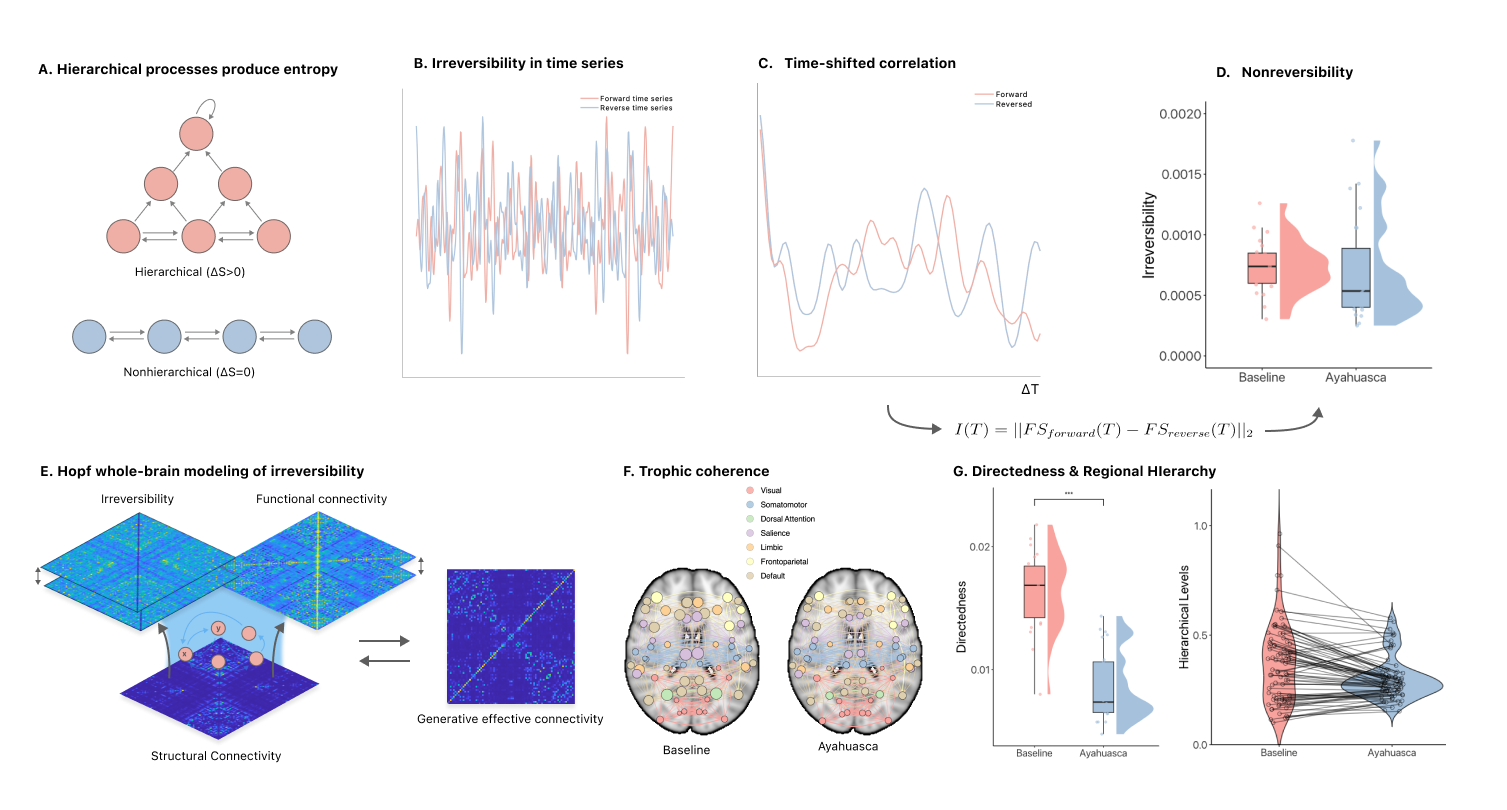
\includegraphics[width=\textwidth]{images/Figure 1.png}
    \caption[Trophic coherence provides causal insights into
the functional hierarchical organization of the brain on drugs]{Trophic coherence provides causal insights into
the functional hierarchical organization of the brain on psychedelics and cannabis. The
figure shows the overall methodological flow presented in this present
study. (A). Participants in three datasets (ayahuasca, DMT, chronic and occasional use of cannabis) were scanned during peak experiences with fMRI (see Methods for acquisition details). BOLD timeseries were extracted after preprocessing. 
(B). Hierarchical processes produce entropy via
irreversible flow of information. Non-hierarchical systems are in
detailed balance and fully reversible, whereas hierarchical systems
break detailed balance. Irreversibility in time-series can be extracted from the
asymmetry between forward and reversed timeseries, shifted in time.
(C) Irreversibility is computed as mutual information, represented by the
absolute quadratic difference, between the time-shifted pairwise
correlation of the forward and reversed timeseries, across all voxels in
the brain. Irreversibility is given by the IR matrix, and hierarchy is
represented as the variability of asymmetry in underlying causal
interactions for each participant in each condition (see Methods).
(D). The irreversibility and structural
anatomical connectivity derived from diffusion tensor imaging (DTI) are used to fit a whole-brain Hopf model, estimating the effective connectivity of irreversibility (see Methods).
(E). The hierarchical influence of each
region in the brain over others (left, right) and the overall trophic coherence, or directedness, of
hierarchical organization (middle), are given through trophic coherence (see Methods). Wilcoxon signed-rank test, middle panel. Non-parametric
two-sample permutation-based test followed by False Discovery Rate,
right panel. (* p\textless0.05; ** p\textless0.01; *** p\textless0.001)}
    \label{fig:overview}
\end{figure}

\section{Irreversibility}
To determine the effects of ayahuasca, DMT, and
cannabis on BOLD fMRI-derived brain hierarchy, 
we first computed irreversibility, an estimate of
production entropy. Irreversibility provides a quantification of how the environment is differentially
driving brain dynamics out of equilibrium depending on the underlying
brain state \parencite{Deco2022,Kringelbach2023}. This is especially relevant within the
context of the psychedelic experience and associated changes in brain
dynamics from long-term use as psychedelics are known to modulate
sensitivity to the environment and extrinsic stimuli, which is
consistent with the role of serotonergic neurotransmission in
environmental sensitivity regulation \parencite{Branchi2011,Carhart-Harris2017}.

We analyzed irreversibility over an 8-minute period after the injection
of DMT or placebo, \textasciitilde12-minute period 1h after the oral
ingestion of ayahuasca, and 6-minute period beginning 15 minutes after
inhalation of cannabis or placebo. The ideal time delay was calculated by finding the value that most effectively discriminated between conditions (see Figure \ref{fig:tau}). Compared
with baseline and placebo conditions, irreversibility was found to be
reduced significantly for DMT (Z=2.79, d = 1.05 [0.32 1.77], p = 0.0052)  and chronic use of
cannabis (Z=2.79, d= 1.05 [0.32 1.77], p = 0.0052) across the whole brain (Figure \ref{fig:ir}a).
Non-significant trends toward decrease were found for ayahuasca (p = 0.41) and
occasional use of cannabis (p = 0.14). A measurement of hierarchy was derived from
the standard deviation of irreversibility for each subject (Figure \ref{fig:ir}b). These results suggest that DMT and chronic
use of cannabis decrease the weight of extrinsic dynamics, or the
environment, on intrinsic brain dynamics.

\begin{figure}[h!]
    \centering
    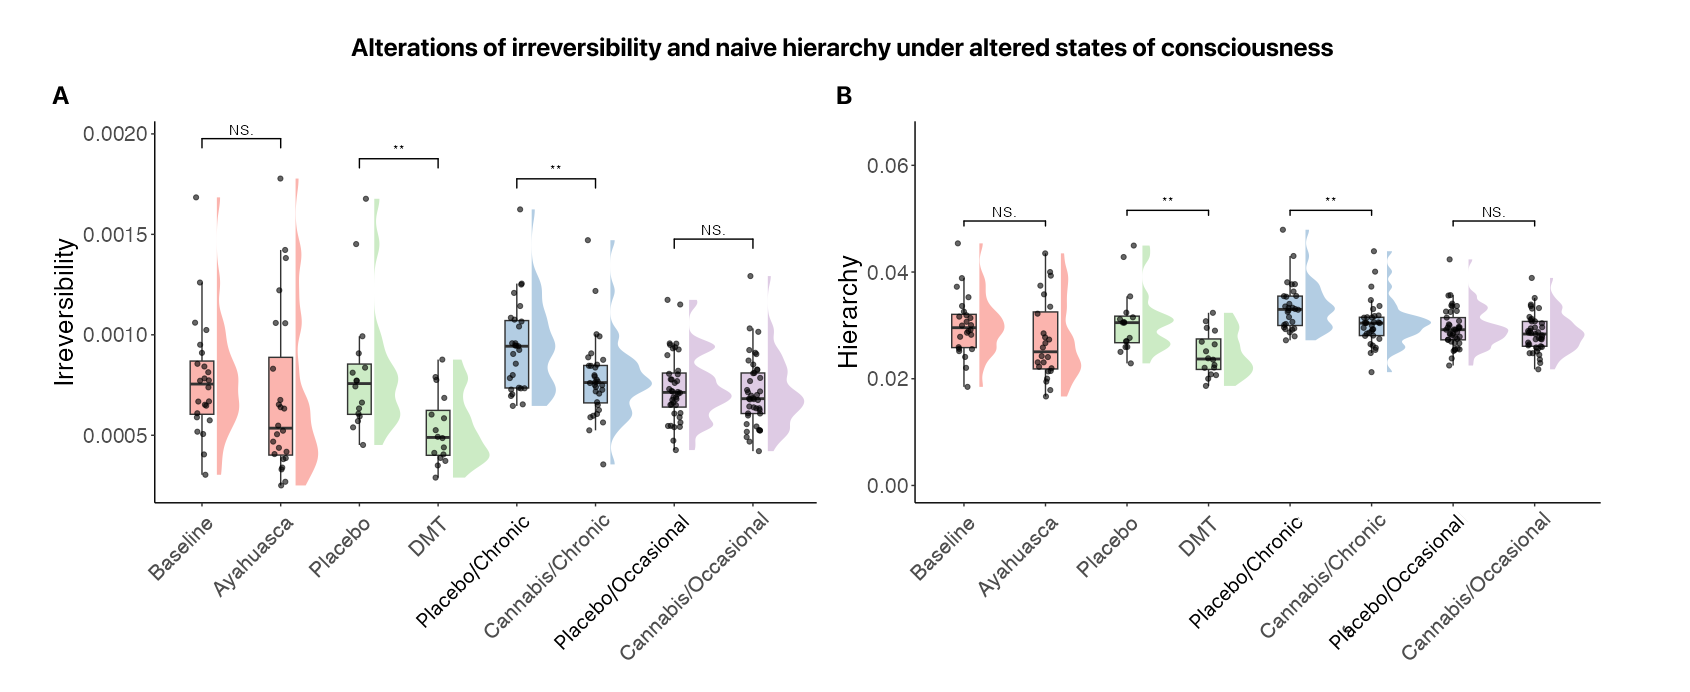
\includegraphics[width=\textwidth]{images/Figure 2_ Nonreversibility.png}
    \caption[Irreversibility and hierarchy of global brain dynamics under
different substances.]{Irreversibility and hierarchy of global brain dynamics under
different substances. (A) Global irreversibility across 80
regions of the DBS80 for ayahuasca, DMT, chronic use of cannabis, and
occasional use of cannabis. Significant decreases,
as evaluated by non-parametric Wilcoxon signed-rank test, were found for DMT>Placebo (Z=2.79, d = 1.05 [0.32 1.77], p = 0.0052) and the
chronic use of cannabis (Z=2.79, d= 1.05 [0.32 1.77], p = 0.0052) , but not occasional use (p = 0.14). A nonsignificant trends
toward decrease in irreversibility was found for ayahuasca (p = 0.41) (B) Similar results were found for
a simple measure of hierarchy, defined as the standard deviation of
irreversibility. Significant differences were found for the change in
irreversibility from placebo to DMT (Z = 2.74, d = 1.14 [0.40 1.86], p = 0.0061), and from baseline to acute cannabis
experience for chronic users (Z = 2.32, d = 0.69 [0.17 1.20], p = 0.02). Nonsignificant decreases in hierarchy were
found for ayahuasca (p = 0.15) and occasional users of cannabis (p = 0.21). (* p\textless0.05;
** p\textless0.01; *** p\textless0.001).}
    \label{fig:ir}
\end{figure}

\section{Trophic coherence of altered states of consciousness}
This first-pass analysis showed that changes in irreversibility, an indirect measure of hierarchy,
are present under both psychedelic and cannabis conditions. We further
examined changes in hierarchy by analyzing the effective connectivity
through whole-brain modelling with generative effective connectivity (GEC) \parencite{Kringelbach2023}. Irreversibility provides information about whether or not hierarchical, or directional, information flow exists between two regions, but does not inform one of which direction that information is moving in. The framework presented here,
first implemented by \textcite{Deco2022}, is less
computationally expensive than alternatives including direct estimation
of the entropy rate through methods like transfer entropy for measuring
Granger causality, and deep learning models \parencite{Deco2021a,Lynn2021,SanzPerl2021,Seif2021}.
Furthermore, this framework has been shown to estimate precise
signatures of different brain states in both electrocorticography (ECoG) data
from non-human primates, including awake, deep sleep, and anesthesia, as
well as differentiating between tasks, rest, and movie-watching in
humans \parencite{Deco2022,Kringelbach2023}.

The model-free quantification of the level of irreversibility is used as
a basis by which to fit a causal, mechanistic whole-brain model, which
provides the effective weighting of the existing structural connectivity
as derived from diffusion tensor imaging \parencite{Friston2003}.
Here, we derived anatomical connectivity from the Human Connectome
Project with 32 participants. This presents a limitation, as
anatomical connectivity is known to vary across individuals and may
result in a less accurate fit to functional connectivity and
irreversibility \parencite{Mueller2013}. The whole-brain model adapts the
strength of existing anatomical connectivity by altering conductance
value parameters in order to optimize connectivity. Iterative estimation of the GEC with
pseudo-gradient descent optimization allows for fitting to the
empirical irreversibility covariance matrix, minimizing the mean-squared
error between empirical and simulated functional connectivity matrices
and the irreversibility covariance matrices. This model, in turn, allows
for evaluation of the generative mechanisms creating hierarchy within
conditions and, importantly, the hierarchical reconfiguration between conditions. A Hopf oscillator model was used as it has previously been shown it
provides the best fit \parencite{Deco2017c, Deco2019a,Deco2017b, Kringelbach2023}. Deviations between empirical and optimized, convergent
simulated functional connectivity and respective covariance matrices are
available in Supplemental Figure \ref{fig:fits}.

The extent to which one region orchestrates the activity of others is
evaluated through summation of the in-degree and out-degree across each region in the brain. As can be seen in Figure \ref{fig:gecrender}, this measure of orchestration varies significantly across conditions. Under the long-term users of ayahuasca, orchestration was found to be most significant in the bilateral pre- and post-central, insula, and superior temporal, as well as the superior frontal gyrus. Under DMT, the insula was less well-connected, though bilateral precuneus became more connected. Under chronic use of cannabis, significant orchestrators were the bilateral isthmus cingulate and rostral anterior cingulate, as well as the bilateral insula. Similarly, bilateral isthmus cingulate and rostral anterior cingulate were primary orchestrators of functional organization under the occasional use of cannabis, as well as the bilateral insula. To complement the analysis of information flow between different regions
captured by the GEC matrix under altered states of consciousness, we
decomposed all brain regions into their canonical resting-state networks
and evaluated changes between baseline or placebo and
drug conditions on orchestration, characterized by the sum of
the in-degree and out-degree, or incoming and outgoing information, from
each network \parencite{Yeo2011}. Figure \ref{fig:gecrender}c details the modulation of
resting-state network orchestration by ayahuasca, DMT, and cannabis.

Regional and network-level orchestration provides information about connectivity changes, but the degree to which a region orchestrates global brain activity is not directly a measure of hierarchy. To better examine the effects of chronic and occasional use of
psychedelics and cannabis on the functional, hierarchical organization
of the brain, we applied trophic coherence to the effective connectivity
derived from the GEC, utilizing the degree of orchestration for each region. Trophic coherence, which we call directedness to differentiate from the method itself, is primarily a measure of how neatly nodes
in a network fall into distinct levels, which is analyzed by the
standard deviation of the distribution of height differences along edges \parencite{Johnson2014,MacKay2020}. The measure was first
applied to ecological food webs in an attempt to better understand the
stability of networks, but it can be applied to any directed network. Previously, it was used to model the coherence of social systems, including dictatorships, military regimes, and anarchy, which found that rigid, hierarchical social systems tend to have higher directedness than democracies or anarchy \parencite{Pilgrim2020}. That is, a higher directedness is associated with a more rigid, stratified network structure.
Here, we consider the effective connectivity of the brain as a directed network, where the degree to which a region orchestrates activity assigns it a trophic, or hierarchical, level that describes its influence over the brain. It is then possible to query the directedness of the network. Networks which display high directedness are clearly defined with regard to each nodes influence over others and are highly stratified. The corollary is that networks with low directedness are highly disordered and lack clearly defined influence relations.

\begin{figure}[h]
    \centering
    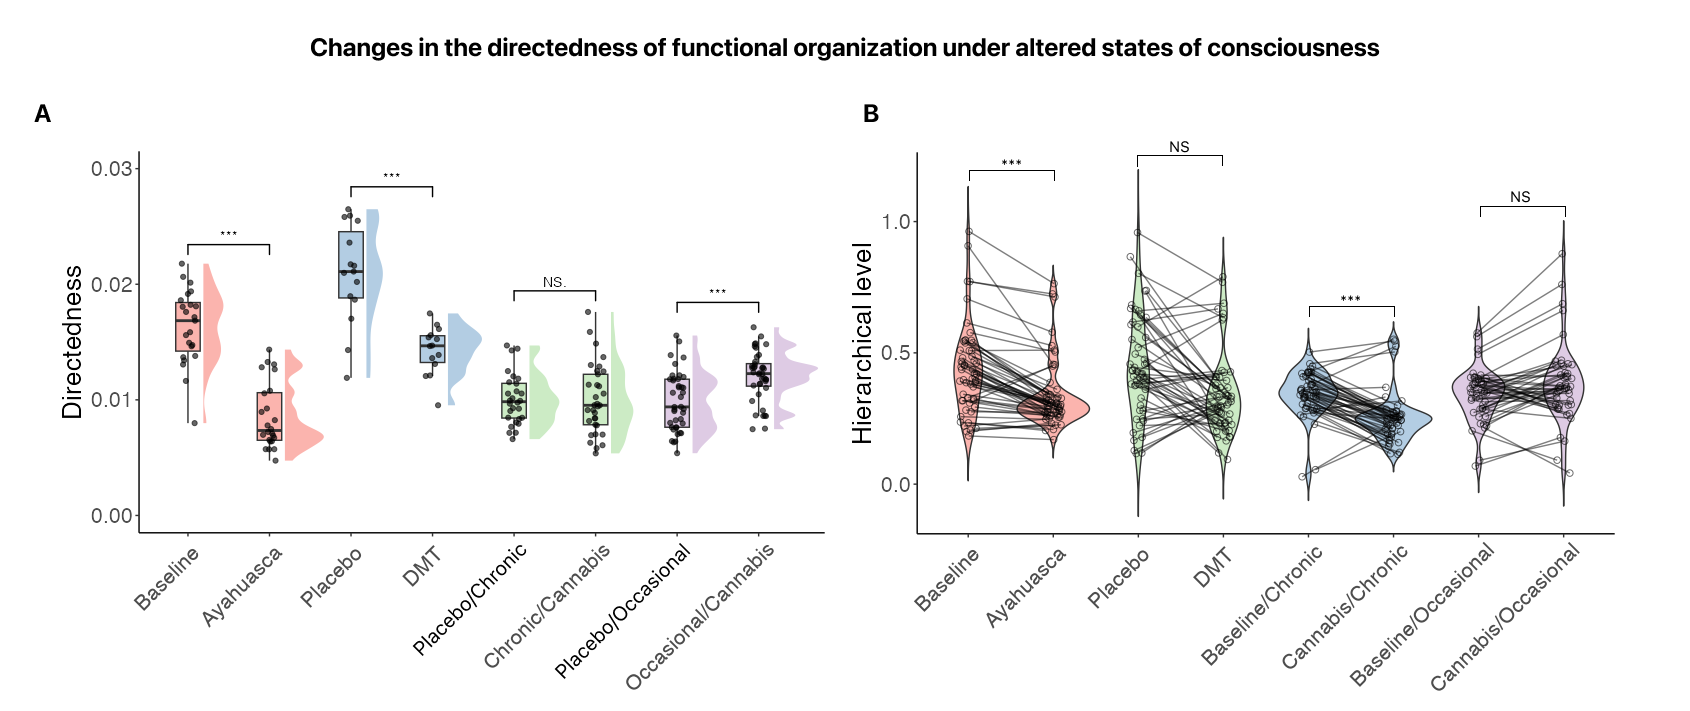
\includegraphics[width=\textwidth]{images/Figure 3_ Trophic coherence.png}
    \caption[Changes in directedness of hierarchical organization under altered state s of consciousness]{Changes in the directedness of functional organization under altered
states of consciousness. (A) Changes in directedness of the
effective connectivity between baseline and placebo and drug conditions.
Compared with baseline, directedness under ayahuasca (t = -8.92, d = 2.50 [1.73 3.26], p = 2.015e-11) and DMT significantly
decreased (d = 0.82 [0.10 1.54], p = 0.010). Interestingly, baseline directedness was much higher for participants in the DMT dataset. Nonsignificant trend
toward decrease was found for the chronic use of cannabis (p = 0.52), while a
significant increase in directedness was found for the occasional use of
cannabis (Z = -3.83, d = -0.91 [-1.36 -0.45], p = 1.28e-4). (B) Changes in trophic levels
after 10,000 iteration non-parametric permutation testing (threshold =
0.01, FDR correction threshold = 0.2). Under ayahuasca, most regions tend to decrease in hierarchical level, while both trends exist for DMT.}
    \label{fig:TC}
\end{figure}

We first analyzed the changes in directedness of the functional
organization of the brain under different states of consciousness, as
well as changes in the individual trophic levels for each region in
the brain from baseline or placebo to drug condition. In Figure \ref{fig:TC}a, it
can be seen that directedness, a direct measure of hierarchical organization,
significantly decreases under ayahuasca (t = -8.92, d = 2.50 [1.73 3.26], p = 2.015e-11) and DMT (d = 0.82 [0.10 1.54], p = 0.010).
In contrast, the occasional use of cannabis resulted in a significant
increase in the directedness of the brain's functional hierarchical
organization (Z = -3.83, d = -0.91 [-1.36 -0.45], p = 1.28e-4), while chronic use of cannabis had no
effect (p = 0.52), possibly due to tolerance \parencite{Ramaekers2022}. Due to differences in study design,
fMRI equipment, and acquisition and preprocessing techniques it is not
possible to make statistical comparisons against conditions. However, we
were uniquely positioned to make inferences about the nature of chronic
and occasional use of psychedelics and cannabis. We also examined changes in hierarchical levels
for each of 80 regions with a 10,000 iteration non-parametric permutation test, followed
by a second permutation test between mean hierarchical level changes across regions between conditions.
In Figure \ref{fig:TC}b, alterations in the hierarchical levels within regions across conditions can be seen. Alterations in directedness
can be considered as a change in the variance of hierarchical levels across conditions.
While directedness decreased significantly for DMT, hierarchical levels varied with regard
to their change in influence. For ayahuasca and occasional use of cannabis, most levels decreased greatly, with the exception
of a few at the bottom of the hierarchy. A similar pattern was seen for the chronic and occasional use of cannabis, where
regions at the bottom and top of the hierarchy tended to increase in influence.

While the measure of orchestration provides a measure of the connectedness of regions, it does not \textit{a priori}
necessitate alterations in hierarchy. 
Trophic coherence, in contrast, provides direct access to
examining alterations in the functional hierarchical organization of the brain. Figure 
\ref{fig:tcrender} details the trophic levels which describe 
the degree of influence a brain region holds for each 
condition. As can be seen in Figure \ref{fig:tcrender}a, 
variability in trophic levels is visually distinct for the chronic and 
occasional use of cannabis versus ayahuasca and DMT. Considerable variability under cannabis for occasional users 
differs from the DMT state, whose variability is similar to 
ayahuasca. These results suggest that tolerance and chronicity 
play a different role in the changes in functional organization 
underlying disparate
altered states of consciousness. 

\begin{figure}[h!]
    \centering
    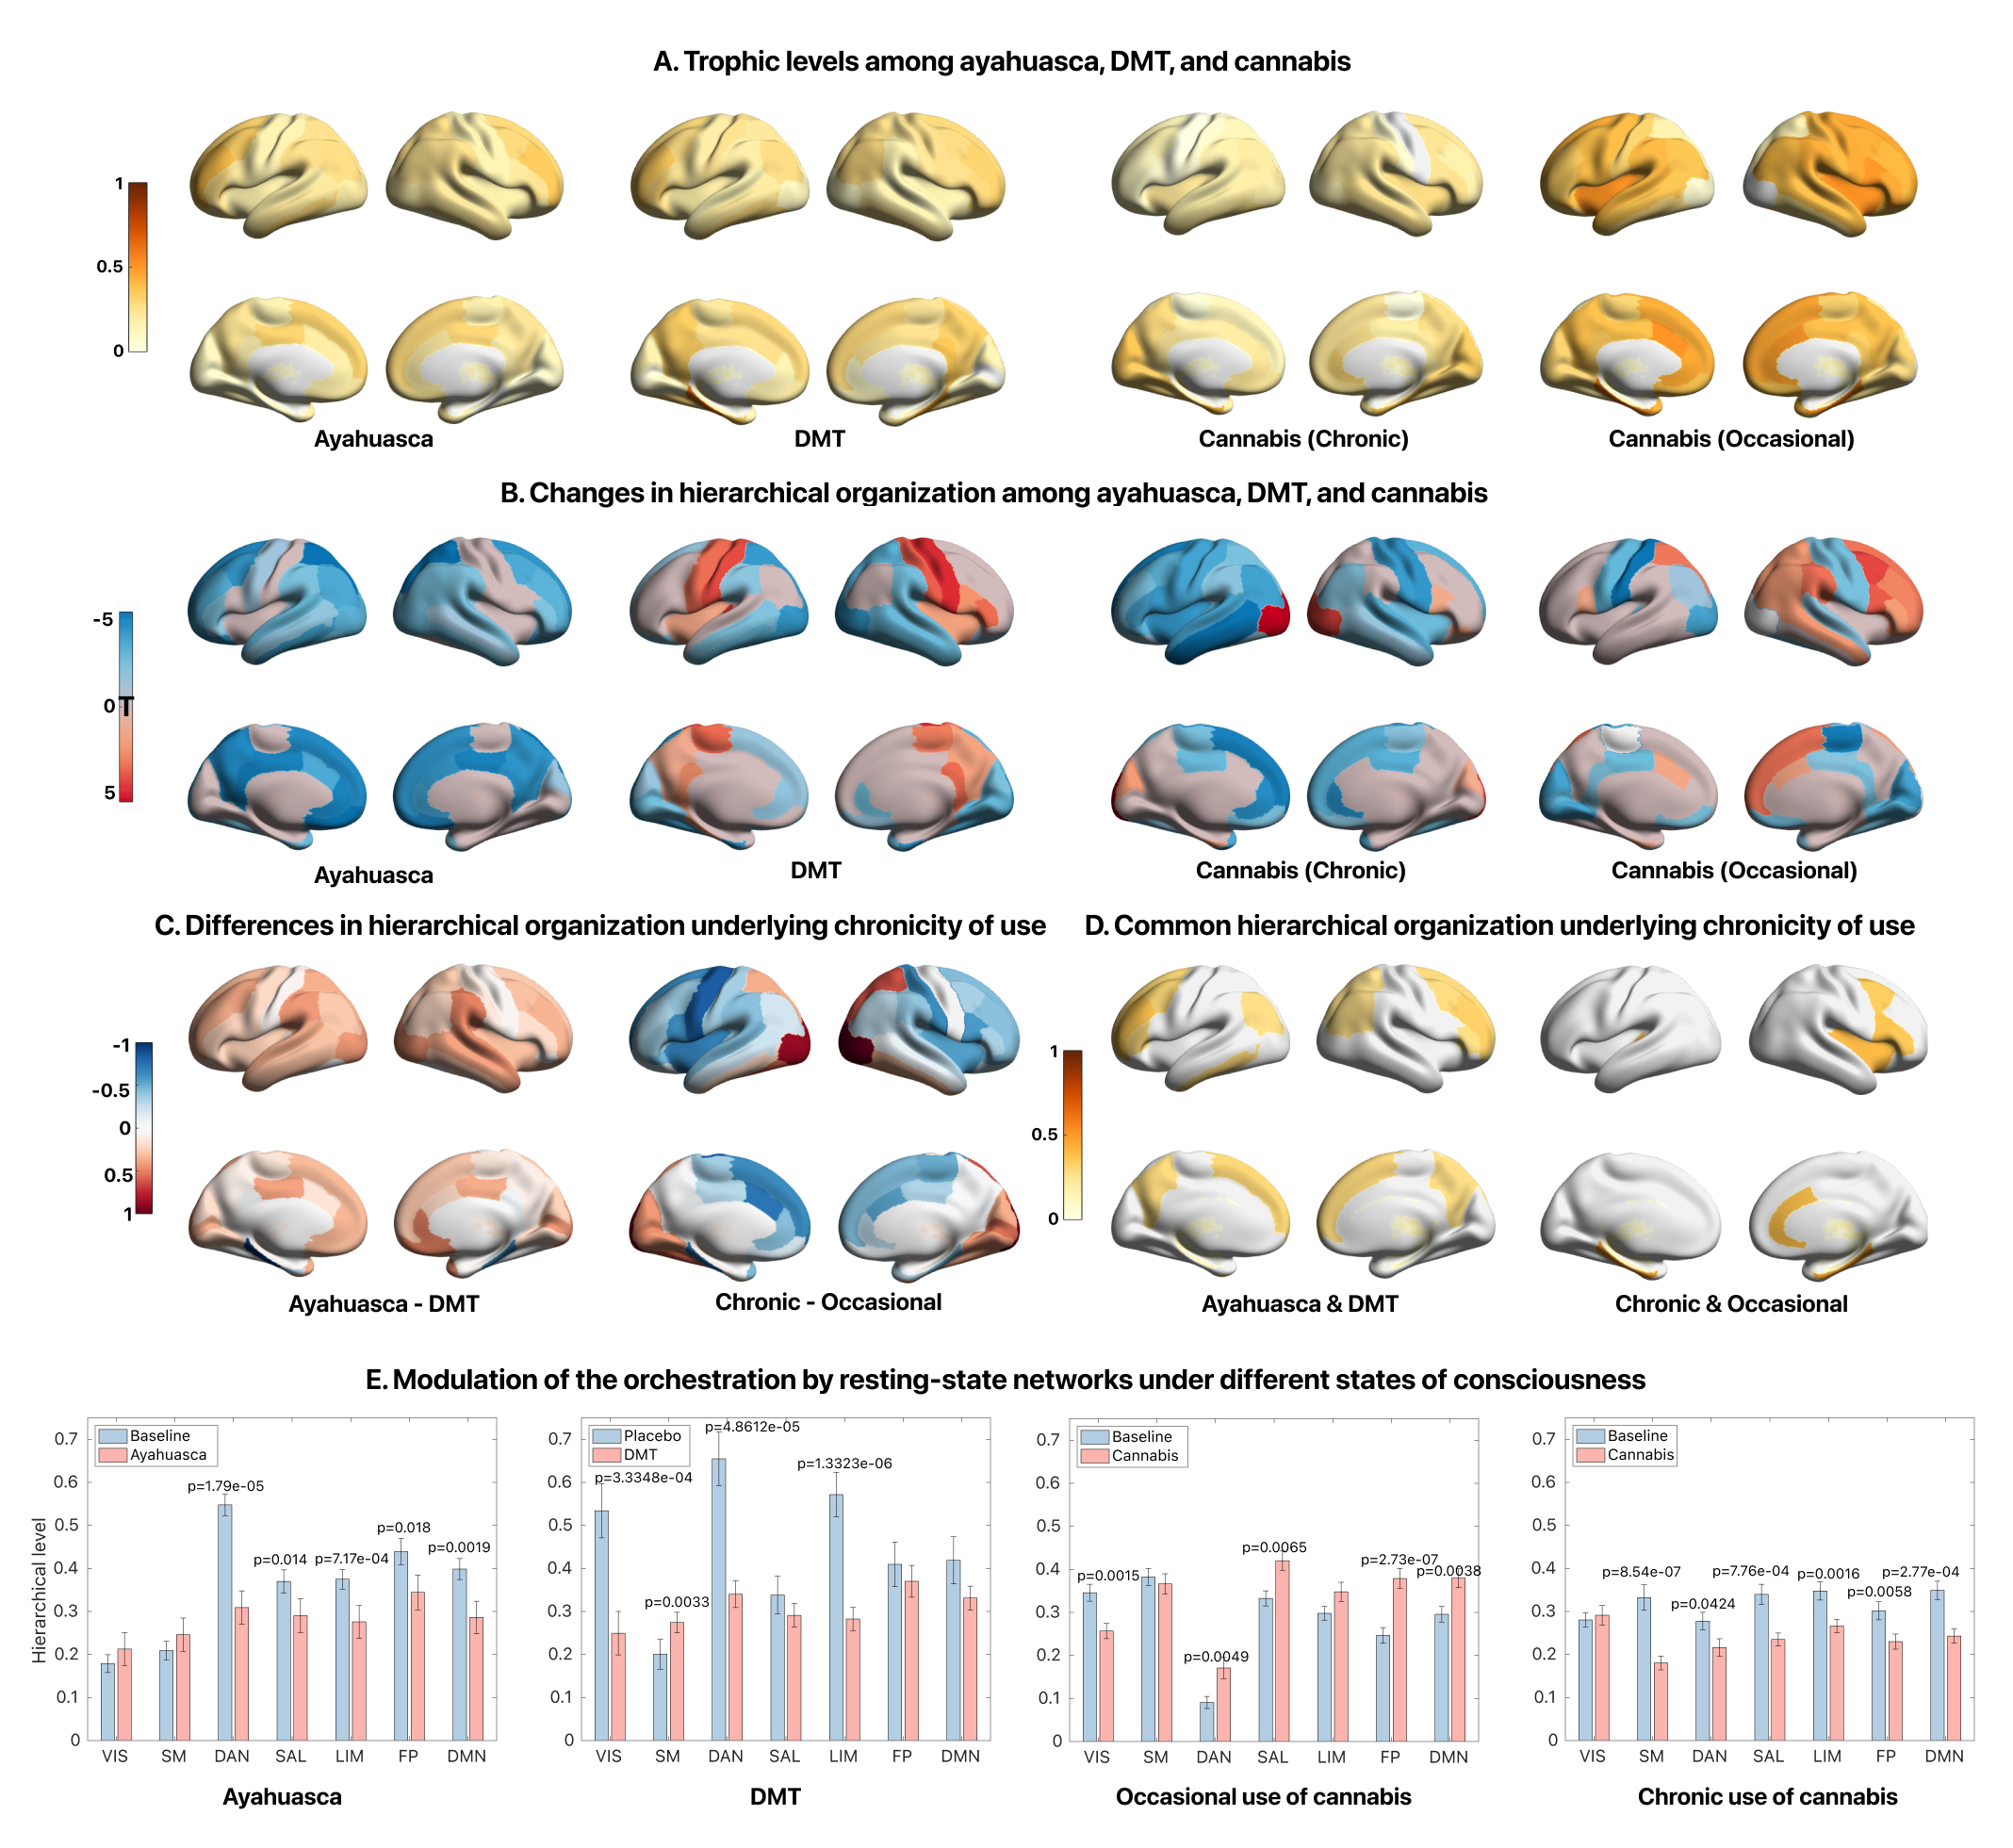
\includegraphics[width=\textwidth]{images/Figure 4_ HL.png}
    \caption[Changes in regional hierarchy orchestrating altered states and their common architecture.]{Changes in
the regional hierarchy orchestrating altered states and their common
hierarchical architecture. (A) Regional hierarchy in acute ayahuasca, DMT,
and cannabis in chronic and occasional users. Significant variability
can be seen for occasional users on cannabis, but not for ayahuasca,
DMT, or cannabis in chronic users. (B) Changes in regional hierarchy
from baseline or placebo to drug condition. Non-parametric 10,000 permutation 
testing with FDR correction identified significant regions. Non-significant regions are shaded grey. (C) Differences in regional hierarchy underlying chronicity of drug use in acute conditions.
Ayahuasca resulted in generally higher regional hierarchy across the cortex than DMT
. With cannabis, occasional use resulted in stronger hierarchy than in chronic use,
except for the occipital cortex. (D) Common regional hierarchy underlying chronicity of drug use in acute conditions. The top 25\% regions in the hierarchy were examined for each drug condition and we found the intersection between
the psychedelics and between cannabis conditions.(E) Modulation of resting-state network hierarchy. Significant decreases (5,000 iteration non-parametric permutation testing, FDR corrected) were found for ayahuasca, DMT, and chronic use of cannabis. Variability in regional hierarchy was found for occasional use of cannabis.}
\label{fig:tcrender}
\end{figure}

We examined changes from baseline or placebo for each condition 
through individual, 10,000 iteration non-parametric permutation 
tests for each region across each condition. It can be seen 
that unlike ayahuasca, DMT resulted in considerable increases in 
bilateral pre- and post-central trophic levels, as well as in 
the bilateral precuneus, paracentral, and isthmus cingulate 
(Figure \ref{fig:tcrender}b). The largest increases 
and decreases in trophic levels for each condition provide 
additional information about the nature of these altered 
states. Interestingly, increases in trophic levels were found 
for subcortical structures under ayahuasca, including the right 
putamen (P < 0.01, FDR corrected) and left globus pallidus externus, not rendered here (P 
< 0.01, FDR corrected). Decreases were seen in 
bilateral superior parietal, left medial orbitofrontal, left 
isthmus cingulate, and left posterior cingulate, consistent 
with previous results \parencite{Timmermann2019,Carhart-Harris2016}. For DMT, increases were found in left and right 
pre-central, left transverse temporal, and left and right post-central (P < 0.01, FDR corrected). Under the chronic 
use of cannabis, decreases in trophic level were seen all 
across the brain, except in left and right medial and lateral 
occipital cortex, left and right thalamus, and right globus 
pallidus internus (P < 0.01, FDR corrected). Decreases 
were found in left middle temporal, left inferior temporal 
cortex, left superior frontal cortex, and the left and right 
rostral anterior cingulate cortices (P < 0.01, FDR 
corrected). For the occasional use of cannabis, increases were 
found in the right subthalamic nucleus, right caudal middle 
frontal, right pars opercularis, right supramarginal, and right 
superior frontal (P < 0.01, FDR corrected). Decreases 
in regional hierarchy were found in the right lateral 
occipital, left and right paracentral, left post-central, and 
right pericalcerine (P < 0.01, FDR corrected). 

We then examined differences in regional hierarchy between acute occasional and chronic use contrasts (Figure \ref{fig:tcrender}c). Ayahuasca generally had higher regional hierarchy across the cortex than did DMT -- in particular, left rostral anterior cingulate cortex and right supramarginal. For Chronic>Occasional, it was found that cannabis in occasional users induced considerably higher regional hierarchy than in chronic users, except in the medial and lateral left and right occipital cortices and superior parietal cortices. After finding differences between conditions, we sought to understand common effects of psychedelics and cannabis across the chronicity of use (Figure \ref{fig:tcrender}d). We took the top 50\% of regions in the hierarchy and evaluated the intersection between them. For ayahuasca and DMT, these common influential regions were in the frontal cortex, as well as left and right superior parietal cortices, superior frontal cortices, and precuneus. For cannabis in chronic and occasional users, these common regions were the right insula, pars opercularis, pars triangularis, and caudal middle frontal, as well as the left anterior cingulate cortex.

\begin{figure}[h!]
    \centering
    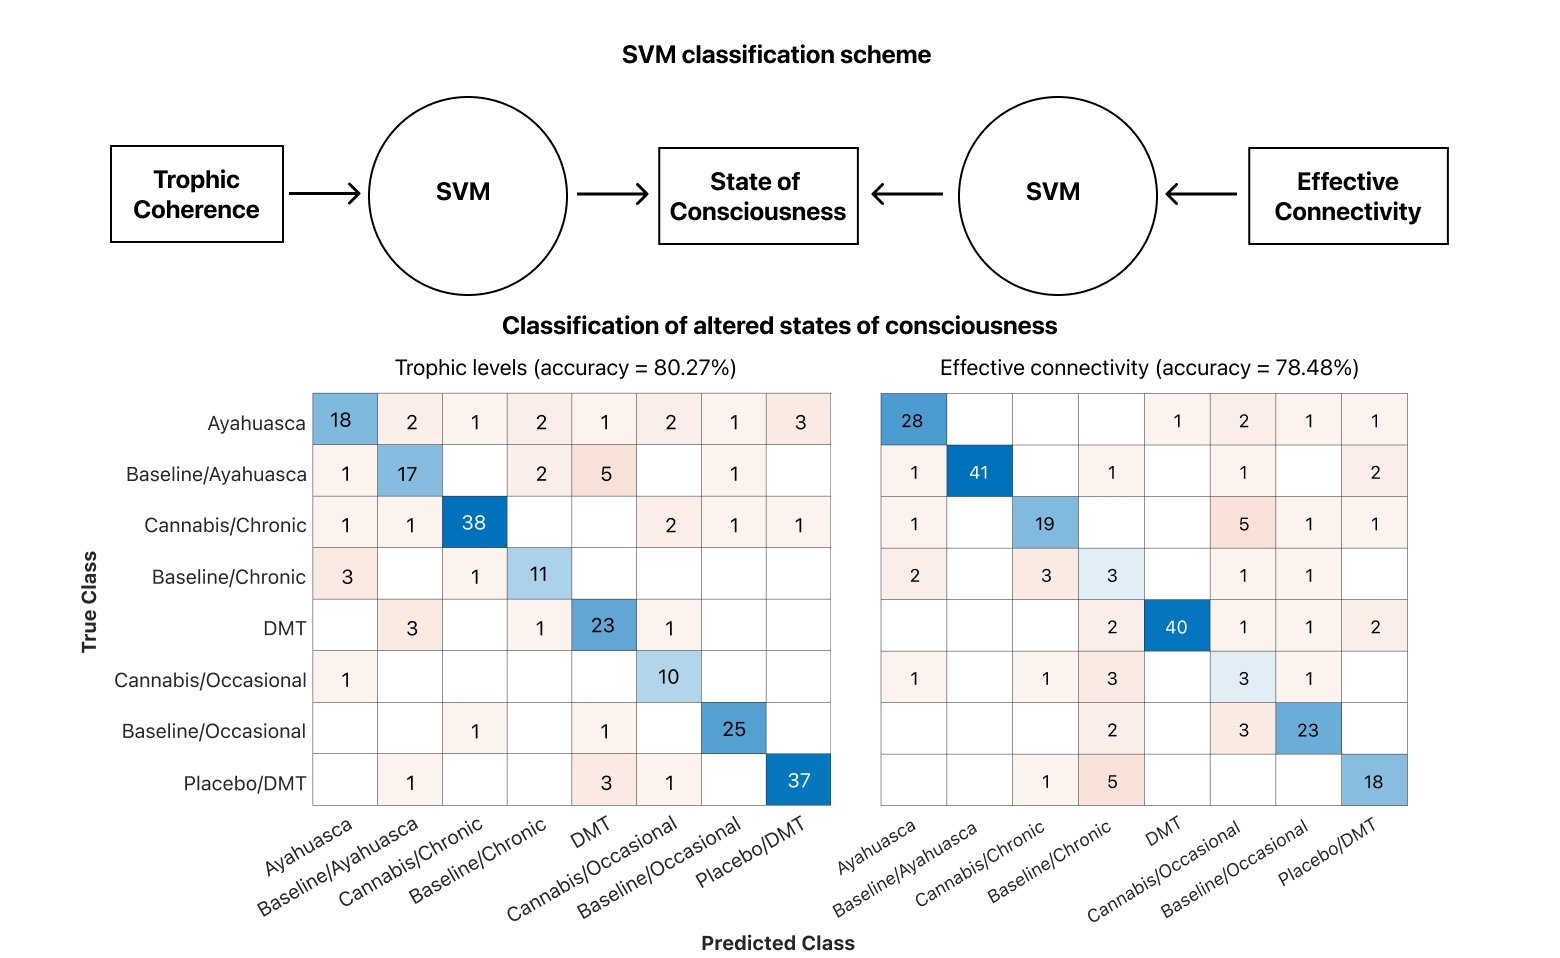
\includegraphics[width=\textwidth]{images/Figure 5 SVM.png}
    \caption[Trophic coherence
is an equivalently performing, simpler discriminator of states of consciousness than
effective connectivity.]{Trophic coherence
is an equivalently performing, simpler discriminator of states of consciousness than
effective connectivity. Figure shows the confusion matrix of the
classification performance (across 5-fold k-fold cross-validation). As
can be seen, the trophic coherence is an equal predictor
of the conscious state condition than effective connectivity (the GEC).
The average performance for trophic coherence is 80.27\%, while the
performance for effective connectivity is slightly lower
(78.48\%).}
    \label{fig:svm}
\end{figure}

To explore changes in the functional integrity of resting-state networks after the administration of psychedelics, we decomposed trophic levels for each region into the resting-state network most associated with that region for changes in trophic level from baseline. Figure \ref{fig:tcrender}e shows the alterations in resting-state network hierarchical influence after the administration of ayahuasca, DMT, and the chronic or occasional use of cannabis. Non-parametric, 10,000 iteration permutation-based hypothesis testing ($\alpha = 0.01$) was followed by FDR correction ($q=0.2$). Significant decreases were seen for ayahuasca and DMT in the dorsal attention and limbic networks, while ayahuasca also significantly decreased the influence of the salience, frontoparietal, and default mode networks (P < 0.05, FDR corrected). DMT, on the other hand, resulted in significant decreases in the visual network and increases in the somatomotor networks (P < 0.05, FDR corrected). Similarly, occasional use of cannabis saw decreases in the visual network, but increased network hierarchy in the dorsal attention, salience, frontoparietal, and default mode networks (P < 0.05, FDR corrected). Lastly, decreases were found across all resting-state networks but the visual network for the chronic use of cannabis (P < 0.05, FDR corrected). Interestingly, ayahuasca induced a non-significant increase in both visual and somatomotor networks, consistent with the idea of a disinhibition of unimodal sensory networks under psychedelics. It is quite a surprise that the visual network hierarchy was significantly higher in resting-state than on DMT.

\begin{figure}[h!]
    \centering
    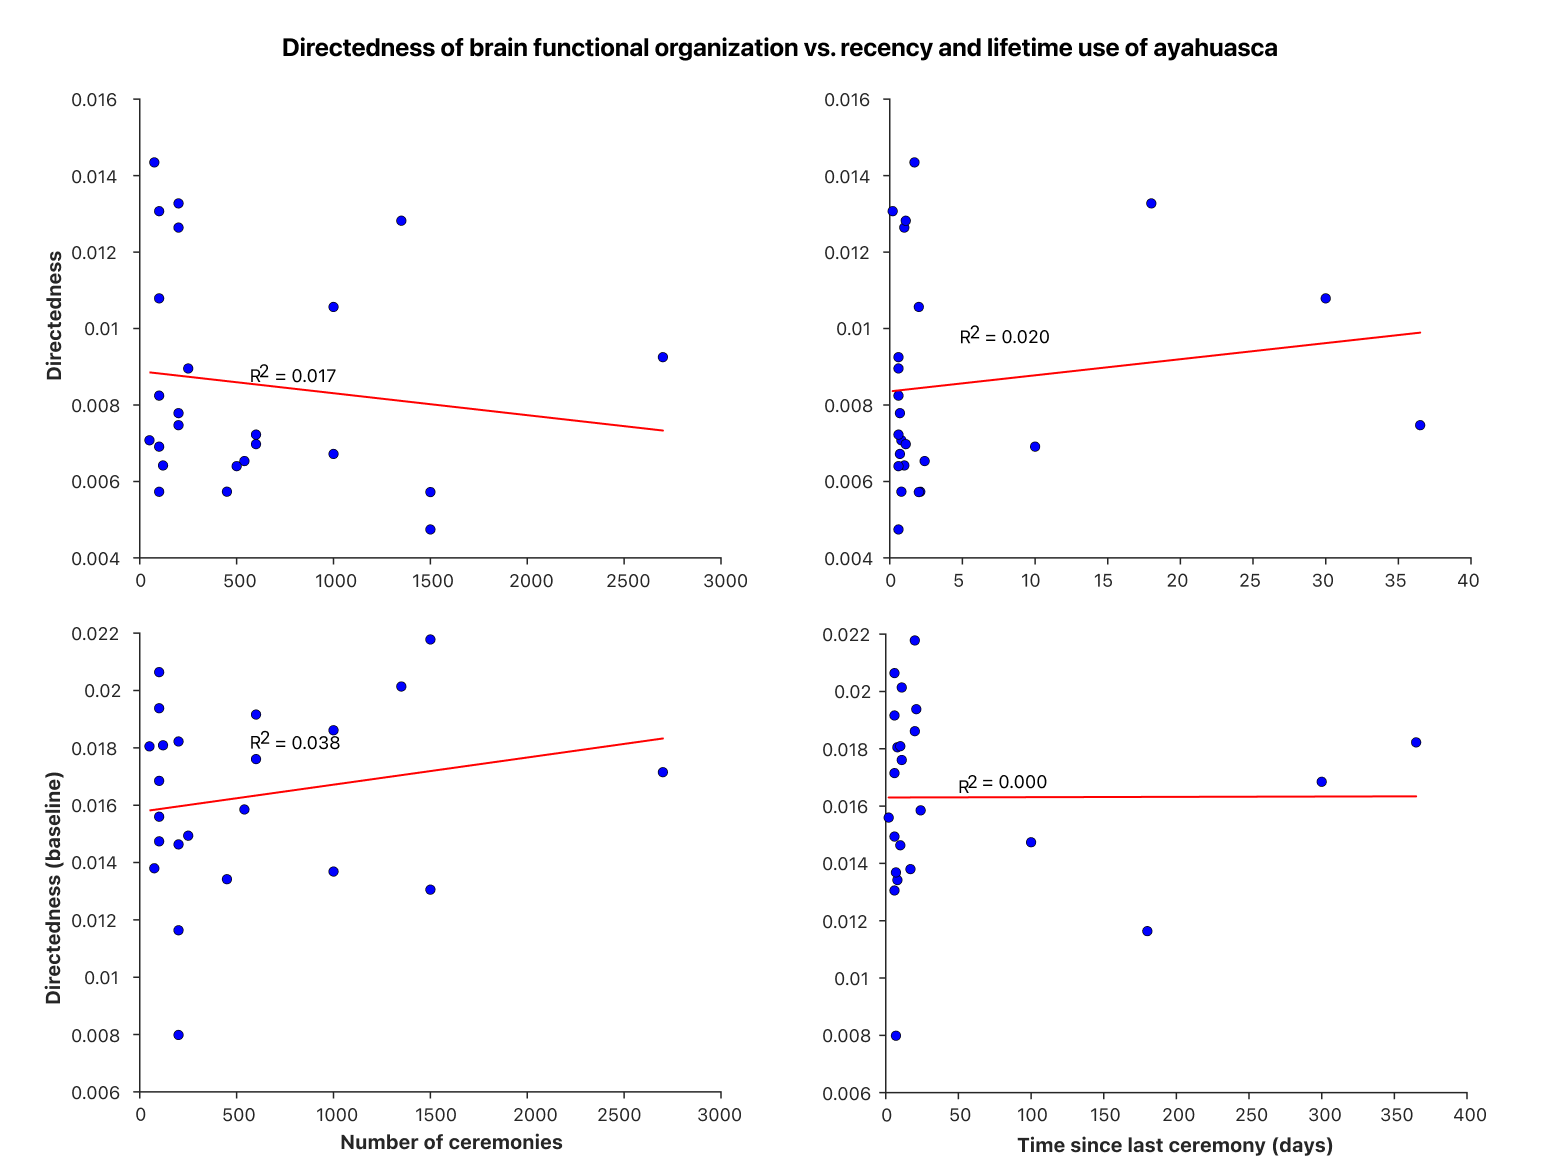
\includegraphics[width=\textwidth]{images/Figure 6_ Correlations between recency.png}
    \caption[Directedness of brain functional organization vs. lifetime use and recency of use.]{Directedness of brain functional organization vs.~lifetime use of
ayahuasca and recency of use. Linear mixed effect models were fit with
directedness (pre- or post-ayahuasca) as the variable to be predicted,
lifetime use or recency as fixed effects, and dosage as a covariate.
Statistical significance was not found for any parameter. Post-ayahuasca
vs number of ceremonies (top-left panel) showed a downward trend with
regard to directedness, with weak correlation (\(R^2=0.017\), p = 0.85).
Post-ayahuasca vs.~time since last ceremony showed an upward trend with
weak correlation (\(R^2=0.020\), p = 0.73). Baseline measures of directedness
(bottom-left panel) showed opposite results against number of
ceremonies, where baseline directedness tended to be higher as the total
number of ceremonies for each participant increased (\(R^2=0.0038\), p = 0.99).
Baseline measures of directedness show no trend with time since last
ceremony (\(R^2=0.000\), p = 0.37).}
    \label{fig:corr}
\end{figure}

Developing a new framework for assessing the direct, causal interactions
orchestrating changes in the functional hierarchical organization of the
brain not only required the evaluation of how these measures compared
with irreversibility and the measure of orchestration of the GEC, but
also to understand whether regional hierarchy can better discriminate
between altered states of consciousness than effective connectivity
alone. We fit a support vector machine (SVM) as a classifier using
either the regional trophic levels or the effective connectivity matrix to
classify the state of consciousness across conditions. Figure \ref{fig:svm} shows
the classification scheme, as well as the confusion matrix
describing the accuracy of models (see Methods). It was found that regional hierarchy
predicted the drug or baseline/placebo condition with 80.27\% accuracy,
while the effective connectivity matrix predicted the condition with 78.48\% accuracy. Directedness, and the global measure of irreversibility are not suitable for this sort of classifier approach -- more features are needed, which is why we use either the subjects-by-region trophic level matrix, or the region-by-by-region irreversibility matrix. In this case, the trophic levels are considered to be less rich in terms of raw data, but the classifier is able to predict equally the state with a small increase in accuracy. Regional hierarchy derived by trophic coherence thus provides a
substantive and accurate dimensionality reduction of the network properties of the irreversibility matrix that captures the functional hierarchical
organization of the brain.

Lastly, we endeavored to better understand the relationship between lifetime use of\\ psychedelics, recency of use, and alterations in functional hierarchical organization. We modeled the linear relationship
between the directedness of networks and lifetime use or recency for
both baseline levels of directedness, as well as altered levels under
ayahuasca. In Figure \ref{fig:corr}, it can be seen that there do not appear to exist
any trends between these measures. Linear mixed-effect models were fit
with post- or pre-ayahuasca directedness as outcome and lifetime use, in
this case number of ayahuasca ceremonies, or recency of use (time since
last ceremony) as fixed effects with the dosage of ayahuasca
administered as a covariate. Despite regional and network-level hierarchy differences between ayahuasca and DMT, a tolerance effect over both short and long timescales does not appear to be present. It may be the case that hierarchical measures do not provide an accurate representation of changes in the brain resulting from long-term use of psychedelics. 
